\subsection{BÀI TẬP TRẮC NGHIỆM}
\ind{PHẦN I.} \inden{Câu trắc nghiệm nhiều phương án lựa chọn. Mỗi câu hỏi học sinh chỉ chọn một phương án.}\\
\setcounter{ex}{0}
\Opensolutionfile{ans}[ans/1H7-B1-1]
\begin{ex}%[1H3B2-1]
	Trong các mệnh đề sau, mệnh đề nào đúng?
	\choice
	{Hai đường thẳng phân biệt cùng vuông góc với một đường thẳng thì song song với nhau}
	{\True Hai đường thẳng phân biệt cùng vuông góc với một mặt phẳng thì song song với nhau}
	{Hai đường thẳng phân biệt cùng vuông góc với một đường thẳng thì vuông góc với nhau}
	{Hai đường thẳng phân biệt cùng song song với một mặt phẳng thì song song với nhau}
	\loigiai{
		Trong các mệnh đề trên thì chỉ có mệnh đề: "Hai đường thẳng phân biệt cùng vuông góc với một mặt phẳng thì song song với nhau" là mệnh đề đúng.
	}
\end{ex}

\begin{ex}%[1H3Y2-1]
	Trong không gian cho đường thẳng $\Delta$ và điểm $O$. Qua $O$ có bao nhiêu đường thẳng vuông góc với $\Delta$?
	\choice
	{$2$}
	{$1$}
	{$3$}
	{\True Vô số}
	\loigiai{
		Qua điểm $O$ có vô số đường thẳng vuông góc với đường thẳng  $\Delta$.
	}
\end{ex}
\begin{ex}%[1H3B2-2]
	\immini[thm]{Cho hình lập phương $ABCD.A'B'C'D'$. Góc giữa hai đường thẳng $AC$ và $B'D'$ bằng
		\choice
		{\True $90^\circ$}
		{$60^\circ$}
		{$30^\circ$}
		{$45^\circ$}}{
		\begin{tikzpicture}[scale=0.7, line join=round, line cap=round]
			\tikzset{label style/.style={font=\footnotesize}}
			\tkzDefPoints{0/0/A,-1.3/-1.1/B,2/-1.1/C}
			\coordinate (D) at ($(A)+(C)-(B)$);
			\coordinate (A') at ($(A)+(0,2.5)$);
			\tkzDefPointsBy[translation=from A to A'](B,C,D){B'}{C'}{D'}
			\tkzDrawPolygon(A',B',B,C,D,D')
			\tkzDrawSegments(B',C' C',D' C,C')
			\tkzDrawSegments[dashed](A,B A,D A,A')
			\tkzDrawPoints[fill=black,size=4](A,B,D,C,A',B',C',D')
			\tkzLabelPoints[above](A',D')
			\tkzLabelPoints[below](A,B,C)
			\tkzLabelPoints[left](B')
			\tkzLabelPoints[right](C',D)
	\end{tikzpicture}}
	\loigiai{
		Do $B'D' \parallel BD$ nên $(AC,B'D')=(AC,BD)=90^\circ$.
	}
\end{ex}

\begin{ex}%[1H3Y2-3]
	\immini[thm]{Cho hình lập phương $ABCD.A'B'C'D'$. Góc giữa hai đường thẳng $BA'$ và $CD$ bằng
		\choice
		{\True $45^\circ$}
		{$30^\circ$}
		{$60^\circ$}
		{$90^\circ$}}{
		\begin{tikzpicture}[line cap=round,line join=round,font=\footnotesize,>=stealth,scale=0.8]
			\fill (0,0) coordinate [label=left:$A$] (A) circle(1pt)
			(4,0) coordinate [label=below right:$B$] (B) circle(1pt)
			(40:2) coordinate [label=left:$D$] (D) circle(1pt)
			(90:3) coordinate [label=left:$A'$] (A') circle(1pt)
			($(B)+(D)$) coordinate [label=right:$C$] (C) circle(1pt)
			($(A')+(B)$) coordinate [label=right:$B'$] (B') circle(1pt)
			($(A')+(C)$) coordinate [label=right:$C'$] (C') circle(1pt)
			($(A')+(D)$) coordinate [label=above:$D'$] (D') circle(1pt);
			\draw (C')--(B')--(A')--(A)--(B)--(C)--(C')--(D')--(A')--(B)--(B');
			\draw [dashed] (A)--(D)--(D') (D)--(C);
	\end{tikzpicture}}
	\loigiai
	{
		\immini
		{Vì $CD\parallel BA$ nên
			\[(BA',CD)=(BA',BA)=\widehat{A'BA}=45^\circ.\]
		}
		{\begin{tikzpicture}[line cap=round,line join=round,font=\footnotesize,>=stealth,scale=0.8]
				\fill (0,0) coordinate [label=left:$A$] (A) circle(1pt)
				(4,0) coordinate [label=below right:$B$] (B) circle(1pt)
				(40:2) coordinate [label=left:$D$] (D) circle(1pt)
				(90:3) coordinate [label=left:$A'$] (A') circle(1pt)
				($(B)+(D)$) coordinate [label=right:$C$] (C) circle(1pt)
				($(A')+(B)$) coordinate [label=right:$B'$] (B') circle(1pt)
				($(A')+(C)$) coordinate [label=right:$C'$] (C') circle(1pt)
				($(A')+(D)$) coordinate [label=above:$D'$] (D') circle(1pt);
				\draw (C')--(B')--(A')--(A)--(B)--(C)--(C')--(D')--(A')--(B)--(B');
				\draw [dashed] (A)--(D)--(D') (D)--(C);
		\end{tikzpicture}}
	}
\end{ex}

\begin{ex}%[1H3K2-4]
	\immini[thm]{Cho hình lập phương $ABCD.A'B'C'D'$ có cạnh bằng $a$. Góc giữa hai đường thẳng $AB'$ và $BC'$ bằng
		\choice
		{ $90^\circ$}
		{\True $60^\circ$}
		{$30^\circ$}
		{$45^\circ$}}{
		\begin{tikzpicture}[scale=1, line join=round, line cap=round]
			\tkzDefPoints{0/0/A,-1.3/-1.1/B,2/-1.1/C}
			\coordinate (D) at ($(A)+(C)-(B)$);
			\coordinate (A') at ($(A)+(0,2.5)$);
			\tkzDefPointsBy[translation=from A to A'](B,C,D){B'}{C'}{D'}
			\tkzDrawPolygon(A',B',B,C,D,D')
			\tkzDrawSegments(B',C' C',D' C,C')
			\tkzDrawSegments[dashed](A,B A,D A,A')
			\tkzDrawPoints[fill=black,size=4](A,B,D,C,A',B',C',D')
			\tkzLabelPoints[above](A',D')
			\tkzLabelPoints[below](A,B,C)
			\tkzLabelPoints[left](B')
			\tkzLabelPoints[right](C',D)
	\end{tikzpicture}}
	\loigiai{
		\immini{
			\begin{itemize}
				\item [$\bullet$] Ta có $AB'\parallel DC'$ nên góc giữa $AB'$ và $BC'$ bằng góc giữa $DC'$ và $BC'$.
				\item [$\bullet$] Xét $\triangle BDC'$ có $BD=DC'=BC'$ (đường chéo hình vuông) nên $\triangle BDC'$ đều.
				\item [$\bullet$] Vậy, $(AB',BC')=(DC',BC')=60^\circ$.
		\end{itemize}}
		{\begin{tikzpicture}[scale=1, line join=round, line cap=round]
				\tkzDefPoints{0/0/A,-1.3/-1.1/B,2/-1.1/C}
				\coordinate (D) at ($(A)+(C)-(B)$);
				\coordinate (A') at ($(A)+(0,2.5)$);
				\tkzDefPointsBy[translation=from A to A'](B,C,D){B'}{C'}{D'}
				\tkzDrawPolygon(A',B',B,C,D,D')
				\tkzDrawSegments(B',C' C',D' C,C' B,C' D,C')
				\tkzDrawSegments[dashed](A,B A,D A,A' B,D)
				\tkzDrawPoints[fill=black,size=4](A,B,D,C,A',B',C',D')
				\tkzLabelPoints[above](A',D')
				\tkzLabelPoints[below](B,C)
				\tkzLabelPoints[left](B')
				\tkzLabelPoints[left](A)
				\tkzLabelPoints[right](C',D)
		\end{tikzpicture}}.}
\end{ex}

\begin{ex}%[1H3B2-3]
	\immini[thm]{Cho tứ diện $ABCD$ có tất cả các cạnh bằng $a$. Số đo góc giữa hai đường thẳng $AB$ và $CD$ bằng
		\choice
		{$60^{\circ}$}
		{$30^{\circ}$}
		{\True $90^{\circ}$}
		{$45^{\circ}$}}{
		\begin{tikzpicture}[scale=.5,font=\footnotesize, line join=round, line cap=round,>=stealth]
			\tkzDefPoints{0/0/B,7/0/C,3/5/A, 2/-2/D}
			\tkzDrawPoints[fill=black](A,B,C,D)
			\tkzLabelPoints[above](A)
			\tkzLabelPoints[below left](B,D)
			\tkzLabelPoints[right](C)
			\tkzDrawSegments(A,B A,C A,D B,D D,C)
			\tkzDrawSegments[dashed](C,B)
	\end{tikzpicture}}
	\loigiai{\vspace{-0.5cm}
		\immini{
			Gọi $M$ là trung điểm của $CD$. \\
			Ta có $\overrightarrow{CD}\cdot\overrightarrow{AM}=\overrightarrow{0}$ và $\overrightarrow{CD}\cdot\overrightarrow{MB}=\overrightarrow{0}$. \\
			$\begin{aligned}
				\text{Do đó } \overrightarrow{CD}\cdot\overrightarrow{AB}
				&=\overrightarrow{CD}\cdot\left(\overrightarrow{AM}+\overrightarrow{MB}\right)\\
				&=\overrightarrow{CD}\cdot\overrightarrow{AM}+\overrightarrow{CD}\cdot\overrightarrow{MB}=\overrightarrow{0}.
			\end{aligned}$\\
			Suy ra $\overrightarrow{AB}\perp \overrightarrow{CD}$ nên số đo góc giữa hai đường thẳng $AB$ và $CD$ bằng $90^{\circ}.$}
		{\begin{tikzpicture}[scale=.4,font=\footnotesize, line join=round, line cap=round,>=stealth]
				\tkzInit[ymin=-3.1,ymax=7.1,xmin=-1.1,xmax=8.1]
				\tkzClip
				\tkzDefPoints{0/0/B,7/0/C,3/6/A, 2/-2/D}
				\tkzDefMidPoint(D,C)\tkzGetPoint{M}
				\tkzDrawPoints[fill=black](A,B,C,D,M)
				\tkzLabelPoints[above](A)
				\tkzLabelPoints[below left](B,D)
				\tkzLabelPoints[below](M)
				\tkzLabelPoints[right](C)
				\tkzDrawSegments(A,B A,M A,C A,D B,D D,C)
				\tkzDrawSegments[dashed](M,B C,B)
	\end{tikzpicture} }}
\end{ex}

\begin{ex}%[1H3B2-4]
	\immini[thm]{Cho tứ diện $ABCD$ có tất cả các cạnh bằng $a$. Gọi $O$ là tâm đường tròn ngoại tiếp tam giác $BCD$. Góc giữa $AO$ và $CD$ bằng bao nhiêu?
		\choice
		{$0^{\circ}$}
		{\True $90^{\circ}$}
		{$30^{\circ}$}
		{$60^{\circ}$}}{
		\begin{tikzpicture}[scale=.5,font=\footnotesize, line join=round, line cap=round,>=stealth]
			\coordinate (B) at (121:5 and 1.5);
			\coordinate (C) at (-110:5 and 1.5);
			\coordinate (D) at (15:5 and 1.5);
			\tkzDefMidPoint(C,D)\tkzGetPoint{M}
			\tkzDefMidPoint(C,B)\tkzGetPoint{N}
			\tkzInterLL(B,M)(D,N)\tkzGetPoint{O}
			\coordinate (A) at ($(O)+(0,6)$);
			\tkzDrawPoints[fill=black](A,B,C,D,M,O)
			\tkzLabelPoints[above](A)
			\tkzLabelPoints[below left](B)
			\tkzLabelPoints[below right](M)
			\tkzLabelPoints[right](D)
			\tkzLabelPoints[below left](C,O)
			\tkzDrawSegments(A,B A,C A,D B,C C,D A,M)
			\tkzDrawSegments[dashed](D,B B,M D,N A,O)
			\draw (B) arc (121:375:5 and 1.5);
			\draw[dashed] (D) arc (15:121:5 and 1.5);
	\end{tikzpicture}}
	\loigiai{
		\immini{
			Gọi $M$ là trung điểm của $CD$.\\
			Vì $ABCD$ là tứ diện đều nên $AM\perp CD$, $OM\perp CD.$ \\
			$\begin{aligned}
				\text{Ta có } \overrightarrow{CD}\cdot\overrightarrow{AO}
				&=\overrightarrow{CD}\cdot\left(\overrightarrow{AM}+\overrightarrow{MO}\right)\\
				&=\overrightarrow{CD}\cdot\overrightarrow{AM}+\overrightarrow{CD}\cdot\overrightarrow{MO}=\overrightarrow{0}.
			\end{aligned}$ \\
			Suy ra $\overrightarrow{AO}\perp \overrightarrow{CD}$ nên số đo góc giữa hai đường thẳng $AO$ và $CD$ bằng $90^{\circ}.$}
		{\begin{tikzpicture}[scale=.5,font=\footnotesize, line join=round, line cap=round,>=stealth]
				\coordinate (B) at (121:5 and 1.5);
				\coordinate (C) at (-110:5 and 1.5);
				\coordinate (D) at (15:5 and 1.5);
				\tkzDefMidPoint(C,D)\tkzGetPoint{M}
				\tkzDefMidPoint(C,B)\tkzGetPoint{N}
				\tkzInterLL(B,M)(D,N)\tkzGetPoint{O}
				\coordinate (A) at ($(O)+(0,6)$);
				\tkzDrawPoints[fill=black](A,B,C,D,M,O)
				\tkzLabelPoints[above](A)
				\tkzLabelPoints[below left](B)
				\tkzLabelPoints[below right](M)
				\tkzLabelPoints[right](D)
				\tkzLabelPoints[below left](C,O)
				\tkzDrawSegments(A,B A,C A,D B,C C,D A,M)
				\tkzDrawSegments[dashed](D,B B,M D,N A,O)
				\draw (B) arc (121:375:5 and 1.5);
				\draw[dashed] (D) arc (15:121:5 and 1.5);
	\end{tikzpicture}}}
\end{ex}
\begin{ex}%[1H3K2-4]
	\immini[thm]{Cho tứ diện $ABCD$ có tất cả các cạnh bằng $a$, $M$ là trung điểm của cạnh $BC$. Khi đó $\cos(AB,DM)$ bằng
		\choice
		{$\dfrac{\sqrt{3}}{2}$}
		{$\dfrac{\sqrt{2}}{2}$}
		{\True $\dfrac{\sqrt{3}}{6}$}
		{$\dfrac{1}{2}$}}{
		\begin{tikzpicture}[scale=.5,font=\footnotesize, line join=round, line cap=round,>=stealth]
			\tkzDefPoints{0/0/B,7/0/D,3/5/A, 2/-2/C}
			\tkzDefMidPoint(B,C)\tkzGetPoint{M}
			\tkzDrawPoints[fill=black](A,B,C,D,M)
			\tkzLabelPoints[above](A)
			\tkzLabelPoints[left](B)
			\tkzLabelPoints[right](D)
			\tkzLabelPoints[below left](M)
			\tkzLabelPoints[below](C)
			\tkzDrawSegments(A,B A,M A,C A,D D,C B,C)
			\tkzDrawSegments[dashed](M,D D,B)
	\end{tikzpicture}}
	\loigiai{
		\immini{
			Giả sử cạnh của tứ diện là $a$.\\
			Tam giác $BCD$ đều $ \Rightarrow DM=\dfrac{a\sqrt{3}}{2}$.\\
			Tam giác $ABC$ đều $ \Rightarrow AM=\dfrac{a\sqrt{3}}{2}$.\\
			Ta có $\cos \left(\overrightarrow{AB},\overrightarrow{DM}\right)=\dfrac{\overrightarrow{AB}\cdot\overrightarrow{DM}}{\left| \overrightarrow{AB}\right|\cdot\left| \overrightarrow{DM}\right|}=\dfrac{\overrightarrow{AB}\cdot\overrightarrow{DM}}{a\cdot\dfrac{a\sqrt{3}}{2}}$\\
			$\begin{aligned}
				\text{Mặt khác}\colon \; \overrightarrow{AB}\cdot\overrightarrow{DM}
				&=\overrightarrow{AB}\left(\overrightarrow{AM}-\overrightarrow{AD}\right)=\overrightarrow{AB}\cdot\overrightarrow{AM}-\overrightarrow{AB}\cdot\overrightarrow{AD}\\
				& =\left| \overrightarrow{AB}\right|\cdot\left| \overrightarrow{AM}\right|\cdot\cos \left(\overrightarrow{AB},\overrightarrow{AM}\right)-\left| \overrightarrow{AB}\right|\cdot\left| \overrightarrow{AD}\right|\cdot\cos \left(\overrightarrow{AB},\overrightarrow{AD}\right) \\ 
				& =\left| \overrightarrow{AB}\right|\cdot\left| \overrightarrow{AM}\right|\cdot\cos 30^{\circ}-\left| \overrightarrow{AB}\right|\cdot\left| \overrightarrow{AD}\right|\cdot\cos 60^{\circ} \\ 
				& =a\cdot\dfrac{a\sqrt{3}}{2}\cdot\dfrac{\sqrt{3}}{2}-a\cdot a\cdot \dfrac{1}{2}=\dfrac{3a^2}{4}-\dfrac{a^2}{2}=\dfrac{a^2}{4}.\\ 
			\end{aligned}$
		}
		{\begin{tikzpicture}[scale=.5,font=\footnotesize, line join=round, line cap=round,>=stealth]
				\tkzInit[ymin=-3,ymax=7,xmin=-1,xmax=8]
				\tkzClip
				\tkzDefPoints{0/0/B,7/0/D,3/6/A, 2/-2/C}
				\tkzDefMidPoint(B,C)\tkzGetPoint{M}
				\tkzDrawPoints[fill=black](A,B,C,D,M)
				\tkzLabelPoints[above](A)
				\tkzLabelPoints[left](B)
				\tkzLabelPoints[right](D)
				\tkzLabelPoints[below left](M)
				\tkzLabelPoints[below](C)
				\tkzDrawSegments(A,B A,M A,C A,D D,C B,C)
				\tkzDrawSegments[dashed](M,D D,B)
		\end{tikzpicture}}\noindent
		$\Rightarrow \cos \left(\overrightarrow{AB},\overrightarrow{DM}\right)=\dfrac{\sqrt{3}}{6}>0\Rightarrow \left(\overrightarrow{AB},\overrightarrow{DM}\right)=\left(AB,DM\right)\Rightarrow \cos \left(AB,DM\right)=\dfrac{\sqrt{3}}{6}.$}
\end{ex}

\begin{ex}%[1H3K2-4]
	\immini[thm]{Cho hình chóp $S.ABC$ có $SA=SB$ và $CA=CB$. Tính số đo của góc giữa hai đường thẳng chéo nhau $SC$ và $AB.$
		\choice
		{\True $90^{\circ}$}
		{$30^{\circ}$}
		{$45^{\circ}$}
		{$60^{\circ}$}}{
		\begin{tikzpicture}[scale=.4,font=\footnotesize, line join=round, line cap=round,>=stealth]
			\tkzInit[ymin=-3.2,ymax=7.2,xmin=-1.2,xmax=8.2]
			\tkzClip
			\tkzDefPoints{0/0/A,7/0/C,3/5/S, 2/-2/B}
			\tkzDrawPoints[fill=black](A,B,C,S)
			\tkzLabelPoints[left](A)
			\tkzLabelPoints[above](S)
			\tkzLabelPoints[below](B)
			\tkzLabelPoints[right](C)
			\tkzDrawSegments(A,B B,C S,A S,B S,C)
			\tkzDrawSegments[dashed](A,C)
			\tkzMarkSegment[color=black,
			pos=0.6,mark=||](S,B)
			\tkzMarkSegment[color=black,
			pos=0.6,mark=||](A,S)
			\tkzMarkSegment[color=black,
			pos=0.6,mark=|](A,C)
			\tkzMarkSegment[color=black,
			pos=0.6,mark=|](B,C)
	\end{tikzpicture}}
	\loigiai{
		\begin{center}
			\begin{tikzpicture}[scale=.4,font=\footnotesize, line join=round, line cap=round,>=stealth]
				\tkzInit[ymin=-3.2,ymax=7.2,xmin=-1.2,xmax=8.2]
				\tkzClip
				\tkzDefPoints{0/0/A,7/0/C,3/6/S, 2/-2/B}
				\tkzDrawPoints[fill=black](A,B,C,S)
				\tkzLabelPoints[left](A)
				\tkzLabelPoints[above](S)
				\tkzLabelPoints[below](B)
				\tkzLabelPoints[right](C)
				\tkzDrawSegments(A,B B,C S,A S,B S,C)
				\tkzDrawSegments[dashed](A,C)
				\tkzMarkSegment[color=black,
				pos=0.6,mark=||](S,B)
				\tkzMarkSegment[color=black,
				pos=0.6,mark=||](A,S)
				\tkzMarkSegment[color=black,
				pos=0.6,mark=|](A,C)
				\tkzMarkSegment[color=black,
				pos=0.6,mark=|](B,C)
			\end{tikzpicture} 
		\end{center}
		$\begin{aligned}
			\text{Xét}\;\; \overrightarrow{SC}\cdot \overrightarrow{AB}&=-\overrightarrow{CS}\cdot \left(\overrightarrow{CB}-\overrightarrow{CA}\right)=\overrightarrow{CS}\cdot \overrightarrow{CA}-\overrightarrow{CS}\cdot \overrightarrow{CB}\\
			& =CS\cdot CA\cdot \cos \widehat{SCA}-CS\cdot CB\cdot \cos \widehat{SCB} \\ 
			& =CS\cdot CA\cdot \dfrac{SC^2+CA^2-SA^2}{2SC\cdot CA}-CS\cdot CB\cdot \dfrac{SC^2+CB^2-SB^2}{2SC\cdot CB} \\ 
			&=\dfrac{SC^2+CA^2-SA^2}{2}-\dfrac{SC^2+CB^2-SB^2}{2}=0~(\text{do\;\;} SA=SB\;\;\text{và\;\;}CA=CB).
		\end{aligned}$
		\\
		Vậy $SC\perp AB$.}
\end{ex}

\begin{ex}%[1H3B2-4]
	Cho hình chóp $S.ABC$ có $AB=AC$ và $\widehat{SAC}=\widehat{SAB}$. Tính số đo của góc giữa hai đường thẳng chéo nhau $SA$ và $BC.$
	\choice
	{$30^{\circ}$}
	{$45^{\circ}$}
	{\True $90^{\circ}$}
	{$60^{\circ}$}
	\loigiai{
		\immini{
			$\begin{aligned}
				\text{Xét}\;\; \overrightarrow{SA}\cdot \overrightarrow{BC}&=\overrightarrow{SA}\cdot \left(\overrightarrow{SC}-\overrightarrow{SB}\right)=\overrightarrow{SA}\cdot \overrightarrow{SC}-\overrightarrow{SA}\cdot \overrightarrow{SB}\\
				&=\left| \overrightarrow{SA}\right|\cdot \left| \overrightarrow{SC}\right|\cdot \cos (\overrightarrow{SA},\overrightarrow{SC})-\left| \overrightarrow{SA}\right|\cdot \left| \overrightarrow{SB}\right|\cdot \cos \widehat{SAB}\\
				&=SA\cdot SC\cdot \cos \widehat{ASC}-SA\cdot SB\cdot \cos \widehat{ASB}.\qquad (1)
			\end{aligned}$}
		{\vspace{-1cm}
			\begin{tikzpicture}[scale=.4,font=\footnotesize, line join=round, line cap=round,>=stealth]
				\tkzInit[ymin=-3.2,ymax=7.2,xmin=-1.2,xmax=8.2]
				\tkzClip
				\tkzDefPoints{0/0/A,7/0/B,3/6/S, 2/-2/C}
				\tkzDrawPoints[fill=black](A,B,C,S)
				\tkzLabelPoints[above](S)
				\tkzLabelPoints[left](A)
				\tkzLabelPoints[right](B)
				\tkzLabelPoints[below](C)
				\tkzDrawSegments(A,C B,C S,A S,B S,C)
				\tkzDrawSegments[dashed](A,B)
		\end{tikzpicture} }
		Ta có $\heva{
			& SA\;\;\text{chung} \\ 
			& AB=AC \\ 
			& \widehat{SAB}=\widehat{SAC} \\}\Rightarrow \triangle SAB=\triangle SAC~\text{(c-g-c)}\Rightarrow \heva{
			& SC=SB \\ 
			& \widehat{ASC}=\widehat{ASB}}\;\;(2)$\\
		Từ $(1)$ và $(2)$, suy ra $\overrightarrow{SA}\cdot \overrightarrow{BC}=0$.\\
		Vậy $SA\perp BC.$}
\end{ex}
\begin{ex}%[1H3K2-4]
	Cho tứ diện $ABCD$ có $AC=\dfrac{3}{2}AD$, $\widehat{CAB}=\widehat{DAB}=60^{\circ} $, $CD=AD$. Gọi $\varphi $ là góc giữa $AB$ và $CD$. Chọn khẳng định đúng.
	\choice
	{$\cos \varphi =\dfrac{3}{4}$}
	{$\varphi =60^{\circ}$}
	{$\varphi =30^{\circ}$}
	{\True $\cos \varphi =\dfrac{1}{4}$}
	\loigiai{
		\begin{center}
			\begin{tikzpicture}[scale=.5,font=\footnotesize, line join=round, line cap=round,>=stealth]
				\tkzInit[ymin=-3.2,ymax=7.2,xmin=-1.2,xmax=8.2]
				\tkzClip
				\tkzDefPoints{0/0/C,7/0/D,3/6/A, 2/-2/B}
				\tkzDrawPoints[fill=black](A,B,C,D)
				\tkzLabelPoints[above](A)
				\tkzLabelPoints[below](B)
				\tkzLabelPoints[right](D)
				\tkzLabelPoints[left](C)
				\tkzDrawSegments(A,B A,C A,D B,C B,D)
				\tkzDrawSegments[dashed](D,C)
				\tkzMarkSegment[color=black,
				pos=0.6,mark=||](A,D)
				\tkzMarkSegment[color=black,
				pos=0.6,mark=||](D,C)
				\tkzMarkAngles[draw=red](C,A,B)
				\tkzMarkAngle[size =0.6,
				mksize=3](B,A,D)
			\end{tikzpicture} 
		\end{center}
		Ta có $\cos \left(AB,CD\right)=\dfrac{\left| \overrightarrow{AB}\cdot \overrightarrow{CD}\right|}{\left| \overrightarrow{AB}\right|\cdot \left| \overrightarrow{CD}\right|}=\dfrac{\left| \overrightarrow{AB}\cdot \overrightarrow{CD}\right|}{AB\cdot CD}.$\\
		$\begin{aligned}
			\text{Mặt khác}\;\; \overrightarrow{AB}\cdot \overrightarrow{CD}&=\overrightarrow{AB}\left(\overrightarrow{AD}-\overrightarrow{AC}\right)=\overrightarrow{AB}\cdot \overrightarrow{AD}-\overrightarrow{AB}\cdot \overrightarrow{AC}\\
			& =\left| \overrightarrow{AB}\right|\cdot \left| \overrightarrow{AD}\right|\cdot \cos (\overrightarrow{AB},\overrightarrow{AD})-\left| \overrightarrow{AB}\right|\cdot \left| \overrightarrow{AC}\right|\cdot \cos (\overrightarrow{AB},\overrightarrow{AC}) \\ 
			& =AB\cdot AD\cdot \cos 60^{\circ}-AB\cdot AC\cdot \cos 60^{\circ} \\ 
			& =AB\cdot AD\cdot \dfrac{1}{2}-AB\cdot \dfrac{3}{2}AD\cdot \dfrac{1}{2}=-\dfrac{1}{4}AB\cdot AD=-\dfrac{1}{4}AB\cdot CD.
		\end{aligned}$\\
		Do có $\cos \left(AB,CD\right)=\dfrac{\left|-\dfrac{1}{4}AB\cdot CD\right|}{AB\cdot CD}=\dfrac{1}{4}$.
		Vậy $\cos \varphi =\dfrac{1}{4}$.}
\end{ex}

\begin{ex}%[1H3B2-3]
	Cho tứ diện $ABCD$ có $AB=CD$. Gọi $I$, $J$, $E$, $F$ lần lượt là trung điểm của $AC$, $BC$, $BD$, $AD$. Góc $(IE,JF)$ bằng
	\choice
	{$30^{\circ}$}
	{$45^{\circ}$}
	{$60^{\circ}$}
	{\True $90^{\circ}$}
	\loigiai{
		\immini{
			Ta có $IF$ là đường trung bình của $\triangle ACD\Rightarrow \heva{
				& IF\parallel CD \\ 
				& IF=\dfrac{1}{2}CD \\}$.\\
			Lại có $JE$ là đường trung bình của $\triangle BCD\Rightarrow \heva{
				& JE\parallel CD \\ 
				& JE=\dfrac{1}{2}CD \\}$.\\
			$\Rightarrow \heva{
				& IF=JE \\ 
				& IF\parallel JE \\}$ $\Rightarrow $ Tứ giác $IJEF$ là hình bình hành.\\
			Mặt khác: $\heva{
				& IJ=\dfrac{1}{2}AB \\ 
				& JE=\dfrac{1}{2}CD \\}$. Mà $AB=CD\Rightarrow IJ=JE$. \\
			Do đó $IJEF$ là hình thoi. Suy ra $\left(IE,JF\right)=90^{\circ}$.}
		{\begin{tikzpicture}[scale=.6,font=\footnotesize, line join=round, line cap=round,>=stealth]
				\tkzInit[ymin=-3,ymax=7,xmin=-1,xmax=8]
				\tkzClip
				\tkzDefPoints{0/0/B,7/0/D,3/6/A, 2/-2/C}
				\tkzDefMidPoint(A,D)\tkzGetPoint{F}
				\tkzDefMidPoint(C,B)\tkzGetPoint{J}
				\tkzDefMidPoint(C,A)\tkzGetPoint{I}
				\tkzDefMidPoint(D,B)\tkzGetPoint{E}
				\tkzDrawPoints[fill=black](A,B,C,I,J,E,F)
				\tkzLabelPoints[above](A)
				\tkzLabelPoints[above left](I)
				\tkzLabelPoints[above right](F)
				\tkzLabelPoints[right](D)
				\tkzLabelPoints[left](B)
				\tkzLabelPoints[below left](J)
				\tkzLabelPoints[below](C,E)
				\tkzDrawSegments(A,C B,C C,D A,D A,B I,F I,J)
				\tkzDrawSegments[dashed](D,B E,J E,F E,I J,F)
				\tkzMarkSegments[color=black,
				pos=0.6,mark=||](A,B C,D)
	\end{tikzpicture}}}
\end{ex}


\begin{ex}%[1H3B2-3]
	Cho tứ diện $ABCD$ có $AC=a, BD=3a$. Gọi $M, N$ lần lượt là trung điểm của $AD$ và $BC$. Biết $AC$ vuông góc với $BD$. Tính $MN$.
	\choice
	{$MN=\dfrac{a\sqrt{6}}{3}$}
	{\True $MN=\dfrac{a\sqrt{10}}{2}$}
	{$MN=\dfrac{2a\sqrt{3}}{3}$}
	{$MN=\dfrac{3a\sqrt{2}}{2}$}
	\loigiai{
		\immini{
			Gọi $P$ là trung điểm của $AB\Rightarrow PN,PM$ lần lượt là đường trung bình của tam giác $\triangle ABC$ và $\triangle ABD$. \\
			Suy ra $\heva{
				& PN=\dfrac{1}{2}AC=\dfrac{a}{2} \\ 
				& PM=\dfrac{1}{2}BD=\dfrac{3a}{2}.}$ \\
			Ta có $AC\perp BD\Rightarrow PN\perp PM$ hay tam giác $\triangle PMN$ vuông tại $P$.\\
			Do đó $MN=\sqrt{PN^2+PM^2}=\sqrt{\dfrac{a^2}{4}+\dfrac{9a^2}{4}}=\dfrac{a\sqrt{10}}{2}.$}
		{\begin{tikzpicture}[scale=.5,font=\footnotesize, line join=round, line cap=round,>=stealth]
				\tkzInit[ymin=-3,ymax=7,xmin=-1,xmax=8]
				\tkzClip
				\tkzDefPoints{0/0/B,7/0/D,3/6/A, 2/-2/C}
				\tkzDefMidPoint(A,D)\tkzGetPoint{M}
				\tkzDefMidPoint(C,B)\tkzGetPoint{N}
				\tkzDefMidPoint(B,A)\tkzGetPoint{P}
				\tkzDrawPoints[fill=black](A,B,C,D,M,N,P)
				\tkzLabelPoints[above](A)
				\tkzLabelPoints[above left](P)
				\tkzLabelPoints[above right](M)
				\tkzLabelPoints[right](D)
				\tkzLabelPoints[left](B)
				\tkzLabelPoints[below left](N)
				\tkzLabelPoints[below](C)
				\tkzDrawSegments(A,C B,C C,D A,D A,B P,N)
				\tkzLabelSegment[pos=.5,left](A,C){  $a$}
				\tkzLabelSegment[pos=.7,above](B,D){  $3a$}
				\tkzDrawSegments[dashed](D,B P,M M,N)
	\end{tikzpicture}}}
\end{ex}

\begin{ex}%[1H3B2-3]
	Cho hình chóp $S.ABCD$ có tất cả các cạnh đều bằng $a$. Gọi $I$ và $J$ lần lượt là trung điểm của $SC$ và $BC$. Tính góc giữa $IJ$ và $CD$.
	\choice
	{$90^{\circ}$}
	{$45^{\circ}$}
	{$30^{\circ}$}
	{\True $60^{\circ}$}
	\loigiai{
		\immini{
			Gọi $O$ là tâm của hình thoi $ABCD$\\
			$\Rightarrow $ $OJ$ là đường trung bình của $\triangle BCD \Rightarrow \heva{
				& OJ\parallel CD \\ 
				& OJ=\dfrac{1}{2}CD.\\}$\\
			Vì $CD\parallel OJ\Rightarrow \left(IJ,CD\right)=\left(IJ,OJ\right)$.\\
			Xét tam giác $IOJ$, có $\heva{
				& IJ=\dfrac{1}{2}SB=\dfrac{a}{2} \\ 
				& OJ=\dfrac{1}{2}CD=\dfrac{a}{2} \\ 
				& IO=\dfrac{1}{2}SA=\dfrac{a}{2} \\}\Rightarrow \triangle IOJ$ đều.\\
			Vậy $\left(IJ,CD\right)=\left(IJ,OJ\right)=\widehat{IJO}=60^{\circ}$.}
		{\begin{tikzpicture}[scale=1, line join=round, line cap=round]
				\tkzDefPoints{0/0/A,-2/-1.6/D,1.6/-1.6/C}
				\coordinate (B) at ($(A)+(C)-(D)$);
				\coordinate (O) at ($(A)!1/2!(C)$);
				\coordinate (S) at ($(O)+(0,3)$);
				\coordinate (I) at ($(S)!1/2!(C)$);
				\coordinate (J) at ($(B)!1/2!(C)$);
				\tkzDrawPolygon(S,B,C,D)
				\tkzDrawSegments(S,C I,J)
				\tkzDrawSegments[dashed](A,S A,B A,D A,C B,D S,O O,I O,J)
				\tkzDrawPoints[fill=black,size=4](D,C,A,B,S,I,J)
				\tkzLabelPoints[above](S)
				\tkzLabelPoints[below](O,C,D,J)
				\tkzLabelPoints[right](B)
				\tkzLabelPoints[left](A,I)
	\end{tikzpicture}}}
\end{ex}

\begin{ex}%[1H3B2-3]
	Cho tứ diện $ABCD$ có $AB$ vuông góc với $CD$. Mặt phẳng $(P)$ song song với $AB$ và $CD$ lần lượt cắt $BC$, $DB$, $AD$, $AC$ tại $M$, $N$, $P$, $Q$. Tứ giác $MNPQ$ là hình gì?
	\choice
	{Hình thang}
	{Hình bình hành}
	{\True Hình chữ nhật}
	{Tứ giác không phải hình thang}
	\loigiai{
		\immini{
			Ta có $\heva{
				& (MNPQ) \parallel AB \\ 
				& (MNPQ)\cap (ABC)=MQ \\} \Rightarrow MQ \parallel AB$. \\
			Tương tự ta có $MN \parallel CD$, $NP \parallel AB$, $QP \parallel CD$.\\
			Do đó tứ giác $MNPQ$ là hình bình hành.\\
			Lại có $MN\perp MQ~(\text{do } AB\perp CD)$.\\
			Vậy tứ giác $MNPQ$ là hình chữ nhật.}
		{\begin{tikzpicture}[scale=.5,font=\footnotesize, line join=round, line cap=round,>=stealth]
				\tkzInit[ymin=-3,ymax=7,xmin=-1,xmax=8]
				\tkzClip
				\tkzDefPoints{0/0/B,7/0/D,3/6/A, 2/-2/C}
				\tkzDefMidPoint(A,D)\tkzGetPoint{P}
				\tkzDefMidPoint(C,B)\tkzGetPoint{M}
				\tkzDefMidPoint(B,D)\tkzGetPoint{N}
				\tkzDefMidPoint(A,C)\tkzGetPoint{Q}
				\tkzDrawPoints[fill=black](A,B,C,D,M,N,P,Q)
				\tkzLabelPoints[above](A)
				\tkzLabelPoints[left](Q)
				\tkzLabelPoints[above right](P)
				\tkzLabelPoints[right](D)
				\tkzLabelPoints[left](B)
				\tkzLabelPoints[below left](M)
				\tkzLabelPoints[below](C,N)
				\tkzDrawSegments(A,C B,C C,D A,D A,B Q,M Q,P)
				\tkzDrawSegments[dashed](D,B N,M P,N)
	\end{tikzpicture}}}
\end{ex}
\begin{ex}%[1H3K2-3]
	Trong không gian cho hai tam giác đều $ABC$ và $ABC'$ có chung cạnh $AB$ và nằm trong hai mặt phẳng khác nhau. Gọi $M$, $N$, $P$, $Q$ lần lượt là trung điểm của các cạnh $AC$, $CB$, $BC'$ và $C'A$. Tứ giác $MNPQ$ là hình gì?
	\choice
	{Hình bình hành}
	{\True Hình chữ nhật}
	{Hình vuông}
	{Hình thang}
	\loigiai{
		\immini{
			Vì $M$, $N$, $P$, $Q$ lần lượt là trung điểm của các cạnh $AC$, $CB$, $BC'$ và $C'A$.\\
			$ \Rightarrow \heva{
				& PQ=MN=\dfrac{1}{2}AB \\ 
				& PQ\parallel AB\parallel MN \\}$ $ \Rightarrow MNPQ$ là hình bình hành.\\
			Gọi $H$ là trung điểm của $AB$.\\
			Vì hai tam giác $ABC$ và $ABC'$ đều nên $\heva{
				& CH\perp AB \\ 
				& C'H\perp AB.}$\\
			Suy ra $AB\perp (CHC')$. Do đó $AB\perp CC'$.\\
			Ta có $\heva{
				& PQ \parallel AB \\ 
				& PN \parallel CC' \\ 
				& AB\perp CC'} \Rightarrow PQ\perp PN$.\\
			Vậy tứ giác $MNPQ$là hình chữ nhật.}
		{\begin{tikzpicture}[scale=.6,font=\footnotesize, line join=round, line cap=round,>=stealth]
				\tkzInit[ymin=-3,ymax=7,xmin=-1,xmax=8]
				\tkzClip
				\tkzDefPoints{0/0/A,7/0/C,5/6/C', 5/-3/B}
				\tkzDefMidPoint(B,C)\tkzGetPoint{N}
				\tkzDefMidPoint(C',B)\tkzGetPoint{P}
				\tkzDefMidPoint(A,C')\tkzGetPoint{Q}
				\tkzDefMidPoint(A,C)\tkzGetPoint{M}
				\tkzDefMidPoint(A,B)\tkzGetPoint{H}
				\tkzDrawPoints[fill=black](A,B,C,C',M,N,P,Q,H)
				\tkzLabelPoints[left](A)
				\tkzLabelPoints[above left](Q)
				\tkzLabelPoints[above](C')
				\tkzLabelPoints[right](C,P)
				\tkzLabelPoints[below right](N)
				\tkzLabelPoints[below left](H)
				\tkzLabelPoints[below](M,B)
				\tkzDrawSegments(A,C' B,C' C,C P,Q P,N C',H A,B C,B C,C')
				\tkzDrawSegments[dashed](Q,M A,C C,H M,N)
	\end{tikzpicture}}}
\end{ex}

\Closesolutionfile{ans}

\ind{PHẦN II.} \inden{Câu trắc nghiệm đúng sai. Trong mỗi ý a), b), c), d) ở mỗi câu, học sinh chọn đúng hoặc sai.}\\
\Opensolutionfile{ans}[ans/1H7-B1-2]

\begin{ex}%[1H8H1-3]
	Trong không gian, cho ba đường thẳng phân biệt $a$, $b$, $c$. Xác định tính đúng sai các mệnh đề sau
	\choiceTF
	{\True Nếu $a\parallel b$ thì $(a,c)=(c,b)$}
	{\True Nếu $c\parallel b$ thì $(a,b)=(a,c)$}
	{Nếu $a\perp c$, $b\perp c$ thì $a\parallel b$}
	{Nếu $a\perp c$ thì $(a,b)=(c,b)$}
	\loigiai{
		\begin{itemchoice}
			\itemch Đúng. 
			\itemch Đúng.
			\itemch Sai. vì $a$, $b$ có thể chéo nhau.
			\itemch Sai. 
		\end{itemchoice}
	}
\end{ex}
%%%==============EX_2============%%%
\begin{ex}%[1H8V1-3]
	\immini[thm]{Cho hình lập phương $ABCD.A'B'C'D'$. Xét tính đúng sai của các khẳng định sau
	\choiceTF
	{\True $BD\parallel B'D'$}
	{\True $\left(AC,B'D'\right)=90^\circ$}
	{\True Tam giác $ACD'$ đều}
	{$\left(AC,A'B\right)=30^\circ$}
}{
\begin{tikzpicture}[scale=0.6, font=\footnotesize, line join=round, line cap=round, >=stealth]
	\def\bc{4} % cạnh BC
	\def\ba{2} % cạnh BA
	\def\gocB{35} % góc B của đáy
	\coordinate[label=below left:$B$] (B) at (0,0);
	\coordinate[label=above left:$A$] (A) at (\gocB:\ba);
	\coordinate[label=below:$C$] (C) at (\bc,0);
	\coordinate[label=right:$D$] (D) at ($(C)-(B)+(A)$);
	\coordinate[label=above left:$A'$] (A') at ($(A)+(90:\bc)$);
	\coordinate[label=left:$B'$] (B') at ($(B)-(A)+(A')$);
	\coordinate[label=above:$C'$] (C') at ($(C)-(A)+(A')$);
	\coordinate[label=right:$D'$] (D') at ($(D)-(A)+(A')$);
	\draw (B')--(B)--(C)--(D)--(D')--(A')--(B')--(C')--(D')--(B') (D')--(C)--(C');
	\draw[dashed] (B)--(A')--(A)--(D) (C)--(A)--(B)--(D) (A)--(D');
	\foreach \diem in {A,B,C,D,A',B',C',D'}	\fill (\diem)circle(1pt);
\end{tikzpicture}}
	\loigiai{\begin{center}
			\begin{tikzpicture}[scale=1, font=\footnotesize, line join=round, line cap=round, >=stealth]
				\def\bc{4} % cạnh BC
				\def\ba{2} % cạnh BA
				\def\gocB{35} % góc B của đáy
				\coordinate[label=below left:$B$] (B) at (0,0);
				\coordinate[label=above left:$A$] (A) at (\gocB:\ba);
				\coordinate[label=below:$C$] (C) at (\bc,0);
				\coordinate[label=right:$D$] (D) at ($(C)-(B)+(A)$);
				\coordinate[label=above left:$A'$] (A') at ($(A)+(90:\bc)$);
				\coordinate[label=left:$B'$] (B') at ($(B)-(A)+(A')$);
				\coordinate[label=above:$C'$] (C') at ($(C)-(A)+(A')$);
				\coordinate[label=right:$D'$] (D') at ($(D)-(A)+(A')$);
				\draw (B')--(B)--(C)--(D)--(D')--(A')--(B')--(C')--(D')--(B') (D')--(C)--(C');
				\draw[dashed] (B)--(A')--(A)--(D) (C)--(A)--(B)--(D) (A)--(D');
				\foreach \diem in {A,B,C,D,A',B',C',D'}	\fill (\diem)circle(1pt);
			\end{tikzpicture}
		\end{center}
		\begin{itemchoice}
			\itemch Đúng. Ta có $BB'\parallel DD'$ và $BB'=DD'\Rightarrow BDD'B'$ là hình bình hành\\ $\Rightarrow BD\parallel B'D'$.
			\itemch Đúng. Vì vậy $(AC,B'D')=(AC,BD)=90^\circ$ (do $AC$ và $BD$ là hai đường chéo hình vuông $ABCD$).
			\itemch Đúng. Ta có $A'D'\parallel BC$, $A'D'=BC\Rightarrow A'BCD'$ là hình bình hành $\Rightarrow A'B\parallel CD'$.
			Vì vậy $(AC,A'B)=(AC,CD')$.
			Gọi $a$ là cạnh của hình lập phương thì\\ $AD'=CD'=AC=a\sqrt{2}$ (đường chéo của hình vuông cạnh $a$).
			Suy ra tam giác $ACD'$ đều nên $(AC,CD')=\widehat{ACD'}=60^\circ$.
			\itemch Sai. Ta có $A'C'\parallel AC$ nên $(AC,A'B)=(A'C',A'B)=\widehat{BA'C'}=60^\circ$.
	\end{itemchoice}	}
\end{ex}

\begin{ex}
	\immini[thm]{Cho hình lập phương ${ABCD.A'B'C'D'}$. Xét tính đúng sai của các khẳng định sau
	\choiceTF
	{ Góc giữa hai đường thẳng ${B'D'}$ và ${B'C}$ bằng ${30^\circ}$ }
	{ \True Góc giữa hai đường thẳng ${B'C}$ và ${AD}$ bằng ${45^\circ}$ }
	{ \True Góc giữa hai đường thẳng ${A'D'}$ và ${CD}$ bằng ${90^\circ}$ }
	{ \True Góc giữa hai đường thẳng ${B'C}$ và ${AD'}$ bằng ${90^\circ}$ }
}{
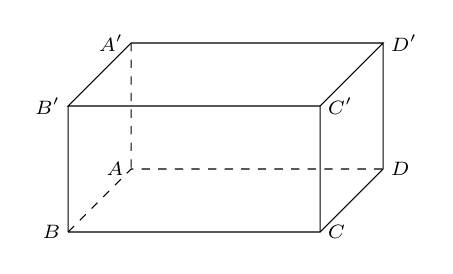
\begin{tikzpicture}[scale=0.8] 
	\begin{scriptsize}
		\coordinate (A) at (0,0)   node at (A) [left] {$A$};
		\coordinate (B) at (-1,-1) node at (B) [left] {$B$};
		\coordinate (C) at (3,-1)  node at (C) [right] {$C$};
		\coordinate (D) at (4,0)   node at (D) [right] {$D$};
		\coordinate (A') at (0,2)   node at (A') [left] {$A'$};
		\coordinate (B') at (-1,1) node at (B') [left] {$B'$};
		\coordinate (C') at (3,1)  node at (C') [right] {$C'$};
		\coordinate (D') at (4,2)   node at (D') [right] {$D'$};
		\draw [dashed] (B)--(A)--(D) (A')--(A);
		\draw (A')--(B')--(C')--(D')--(A') (B')--(B) (C')--(C) (D')--(D);
		\draw (B)--(C)--(D);
	\end{scriptsize}
\end{tikzpicture}}
	\loigiai{ 
		a) Vì tam giác ${B'D'C}$ đều nên $(B'D', B'C)= 60^\circ$.\\ 
		b) $(B'C, AD)= (B'C,BC)=45^\circ$.\\ 
		c) $(A'D', CD)= (A'D',C'D')=90^\circ$.\\ 
		d) $(B'C, AD')= (B'C,BC')=90^\circ$.\\ 
		
}\end{ex}

\begin{ex}%[1H8H1-3]
	Cho tứ diện đều $ABCD$ có cạnh bằng $a$, $M$ là trung điểm cạnh $BC$, $N$ là trung điểm của $AC$. Xét tính đúng sai của các khẳng định sau
	\choiceTF
	{\True $MN\parallel AB$}
	{$MD=ND=\dfrac{a\sqrt{2}}{2}$}
	{\True $(AB,DM)=(MN,DM)$}
	{$\cos (AB,DM)=\dfrac{\sqrt{3}}{3}$}
	\loigiai{\begin{center}
			\begin{tikzpicture}[scale=1, font=\footnotesize, line join=round, line cap=round, >=stealth]
				\def\ac{4.5} % cạnh AC
				\def\ab{2} % cạnh Ab
				\def\h{4} % đường cao
				\def\gocA{45} % góc A của đáy
				\coordinate[label=left:$A$] (A) at (0,0);
				\coordinate[label=below left:$B$] (B) at (-\gocA:\ab);
				\coordinate[label=right:$C$] (C) at (\ac,0);
				\coordinate[label=below right:$M$] (M) at ($(B)!.5!(C)$);
				\coordinate[label=below:$N$] (N) at ($(A)!.5!(C)$);
				\coordinate (G) at ($(A)!2/3!(M)$);
				\coordinate[label=above left:$D$] (D) at ($(G)+(90:\h)$);
				\draw (A)--(B)--(C)--(D)--cycle (M)--(D)--(B);
				\draw[dashed] (A)--(C) (M)--(N)--(D);
				\foreach \diem in {A,B,C,M,N,D}	\fill (\diem)circle(1pt);
			\end{tikzpicture}
		\end{center}
		\begin{itemchoice}
			\itemch Đúng. Gọi $N$ là trung điểm của $AC$ nên $MN$ là đường trung bình của $\triangle ABC$\\ $\Rightarrow \heva{&MN\parallel AB\quad(*)\\& MN=\dfrac{1}{2} AB=\dfrac{a}{2}.}$
			\itemch Sai. Vì $\triangle BCD$ và $\triangle ACD$ là các tam giác đều cạnh bằng $a$ nên $MD=ND=\dfrac{a\sqrt{3}}{2}$.
			\itemch Đúng. Từ $(*)$ suy ra $(AB,DM)=(MN,DM)$.
			\itemch Sai. Xét $\triangle MND$, ta có 
			$$\cos \widehat{DMN}=\dfrac{MN^2+MD^2-ND^2}{2MN\cdot MD}=\dfrac{\left(\dfrac{a}{2}\right)^2+\left(\dfrac{a \sqrt{3}}{2}\right)^2-\left(\dfrac{a\sqrt{3}}{2}\right)^2}{2\cdot \dfrac{a}{2}\cdot \dfrac{a\sqrt{3}}{2}}=\dfrac{\sqrt{3}}{6}>0.$$
			$\Rightarrow \widehat{DMN}$ là góc nhọn.\\
			Vậy $(AB,DM)=(MN,DM)=\widehat{DMN}$ nên $\cos (AB,DM)=\dfrac{\sqrt{3}}{6}$.
	\end{itemchoice}	}
\end{ex}

\Closesolutionfile{ans}

\ind{PHẦN III.} \inden{Câu trắc nghiệm trả lời ngắn.}\\
\Opensolutionfile{ans}[ans/1H7-B1-3]

\begin{ex}%[1H8H1-3]
	Cho hình lăng trụ $ABC.MNP$ có $ABC$ là tam giác vuông tại $B$, $\widehat{ACB}=30^\circ$. Góc $\left(MN, AC\right)$ bằng bao nhiêu độ?\\
	\shortans[oly]{$60$}
	\loigiai{\immini{$\left(MN, AC\right)=\left(AB, AC\right)=\widehat{BAC}=90^\circ-30^\circ=60^\circ$.}
		{\begin{tikzpicture}[>=stealth,line join=round,line cap=round]
				\draw (0,0)coordinate(A)--(-35:1.5)coordinate(B)--(3,0)coordinate(C)--($(C)+(90:3)$)coordinate(P)--($(B)-(C)+(P)$)coordinate(N)--($(A)-(B)+(N)$)coordinate(M)--(P) (A)--(M) (B)--(N);
				\draw[dashed]  (A)--(C);
				\foreach \diem/\vitrin in {A/left,B/below left,C/right,M/left,N/below left,P/right}	\fill (\diem)circle(1pt)node[\vitrin]{$\diem$};
	\end{tikzpicture}}}
\end{ex}

\begin{ex}%[1H3-2.4-2]
	Cho hình chóp $S.ABCD$ có $SA=a, SB=2a, SC=3a, \widehat{ASB}=\widehat{BSC}=60^\circ , \widehat{CSA}=90^\circ $. Gọi $\alpha $ là góc giữa hai đường thẳng $SA$ và $BC$. Tính $\cos \alpha $ (kết quả làm tròn đến 2 chữ số thập phân).\\
	\shortans[oly]{$0,38$}
	\loigiai{
		\begin{align*}
			\cos \alpha &=\left| \cos (\overrightarrow{SA},\overrightarrow{BC}) \right|=\dfrac{\left| \overrightarrow{SA}.\overrightarrow{BC} \right|}{SA.BC}=\dfrac{\left| \overrightarrow{SA}.(\overrightarrow{SC}-\overrightarrow{SB}) \right|}{SA.BC}\\
			&=\dfrac{\left| \overrightarrow{SA}.\overrightarrow{SC}-\overrightarrow{SA}.\overrightarrow{SB} \right|}{SA.BC}=\dfrac{\left| SA.SC.\cos 90^\circ -SA.SB.\cos 60^\circ  \right|}{a.\sqrt{4{a^2}+9{a^2}-2.2a.3a.\cos 60^\circ}}=\dfrac{\sqrt{7}}{7}\approx0,38
		\end{align*}
	}
\end{ex}

\begin{ex}%[1H8C1-3]
	\immini[thm]{
		Một con dốc có dạng hình lăng trụ đứng $ABC.A'B'C'$ (các mặt $AA'C'C$, $AA'B'B$, $BCC'B'$ là các hình chữ nhật; $\triangle ABC$, $\triangle A'B'C'$ là các tam giác vuông) với chiều cao bằng $5\mathrm{~m}$, độ dốc bằng $30^\circ$ so với mặt đất. Biết con dốc rộng $8\mathrm{~m}$. Tính số đo góc (theo đơn vị độ) tạo bởi đường thẳng $A'C$ và $B'C'$. (Làm tròn kết quả đến hàng phần mười)\\
		\shortans[oly]{$47{,}5$}}
	{	\begin{tikzpicture}[line cap=round,line join=round,font=\footnotesize,>=stealth,scale=0.8]
			\coordinate[label=left:$C$] (C) at (0,0);
			\coordinate[label=right:$C'$] (C') at (4,0);
			\coordinate[label=below:$B$] (B) at (1.5,-1.5);
			\coordinate[label=below:$B'$] (B') at ($(C')+(B)-(C)$);
			\coordinate[label=above:$A$] (A) at	($(C)+(1,3)$);
			\coordinate[label=above:$A'$] (A') at	($(C')+(1,3)$);
			\draw (C)--(B)--(A)--cycle (B)--(B')--(A')--(A)--cycle (A')--(B);
			\draw[dashed] (C')--(C) (C')--(B') (C')--(A');
			\foreach \x in {A,B,C,A',B',C'} \draw[fill=red]  (\x) circle (1pt);
	\end{tikzpicture}}
	\loigiai{\immini{
			\begin{itemize}
				\item Vì $ABC.A'B'C'$ là hình lăng trụ đứng nên\\ $BC\parallel B'C'\Rightarrow \left(A'B,B'C'\right)=\left(A'B,BC\right)$.
				\item Xét $\Delta AA'C$ vuông tại $A$, theo định lý Pythagoras ta có\\
				$A'C=\sqrt{AA'^2+AC^2}=\sqrt{5^2+8^2}=\sqrt{89}\mathrm{~m}$.
		\end{itemize}}
		{	\begin{tikzpicture}[line cap=round,line join=round,font=\footnotesize,>=stealth,scale=0.8]
				\coordinate[label=left:$C$] (C) at (0,0);
				\coordinate[label=right:$C'$] (C') at (4,0);
				\coordinate[label=below:$B$] (B) at (1.5,-1.5);
				\coordinate[label=below:$B'$] (B') at ($(C')+(B)-(C)$);
				\coordinate[label=above:$A$] (A) at	($(C)+(1,3)$);
				\coordinate[label=above:$A'$] (A') at	($(C')+(1,3)$);
				\path (A)--(C)node[pos=0.5,black,left]{$5$m};
				\path (B)--(B')node[pos=0.5,black,above]{$8$m};
				\path pic[angle radius=5mm,draw=blue,"$30^\circ$",angle eccentricity=1.5] {angle = A--B--C};
				\draw (C)--(B)--(A)--cycle (B)--(B')--(A')--(A)--cycle (A')--(B);
				\draw[dashed] (C')--(C) (C')--(B') (C')--(A')--(C);
				\foreach \x in {A,B,C,A',B',C'} \draw[fill=red]  (\x) circle (1pt);
		\end{tikzpicture}}\noindent
		\begin{itemize}
			\item Xét $\triangle ABC$ vuông tại $C$, theo hệ thức lượng ta có\\
			$BC=AC\cdot \cot \widehat{ABC}=5\cdot \cot 30^\circ=5\sqrt{3}\mathrm{~m}$ \\
			$AB=\dfrac{AC}{\sin \widehat{ABC}}=\dfrac{5}{\sin 30^\circ}=10\mathrm{~m}$.
			\item Xét $\triangle AA'B$ vuông tại $A$, theo định lý Pythagoras ta có\\
			$A'B=\sqrt{AA'^2+AB^2}=\sqrt{8^2+10^2}=2\sqrt{41}\mathrm{~m}$ 
			\item Xét $\triangle A'BC$ theo định lý cosin ta có
			\[\cos \widehat{A'BC}=\dfrac{A'B^2+BC^2-A'C^2}{2\cdot A'B\cdot BC}=\dfrac{5\sqrt{123}}{82} \Rightarrow \widehat{A'BC}\approx 47{,}5^\circ
			\]
			Vậy góc tạo bởi đường thẳng $A'C$ và $B'C'$ có số đo xấp xỉ bằng $47{,}5^\circ$.
		\end{itemize}
	}
\end{ex}
%%%==============EX_6============%%%
\begin{ex}%[1H8C1-3]
	\immini[thm]{
		Một chiếc thang có dạng hình thang cân cao $6\mathrm{~m}$, hai chân cách nhau $80\mathrm{~cm}$, hai ngọn thang cách nhau $60\mathrm{~cm}$. Thang được dựa vào bờ tường như hình bên. Tính góc tạo giữa đường thẳng chân tường và cạnh cột thang (tính gần đúng theo đơn vị độ)\\
	\shortans[oly]{$89$}}
	{\begin{tikzpicture}[scale=.45, font=\footnotesize, line join=round, line cap=round, >=stealth]
			\definecolor{mauxam}{RGB}{223,221,219}
			\definecolor{xamdam}{RGB}{89,102,112}
			\definecolor{c737d86}{RGB}{115,125,134}
			\definecolor{c656d73}{RGB}{101,109,115}
			\def\buctuongtrai{(0,15) .. controls (1.5,15.3) and (2,14.2) ..
				(2.8,13.5) .. controls (3.5,13.4) and (4,13.5) ..
				(4.5,13.6)-- (6.6,12.6)  --(6.6,.9)--(0,4.5)--cycle}
			\definecolor{gach}{rgb}{0.82, 0.41, 0.12}
			\tikzset{gach/.pic={
					\def\d{1}%Độ dài viên gạch
					\def\r{\d*0.5}% Độ rộng viên gạch
					\def\n{6}
					\def\h{24}
					\foreach \x in {-3,-2,...,\n}
					\foreach \y in {-2,0,...,\h}{
						\draw[fill=gach,draw=gray!60,line width=1pt](\d*\x,\y*\r)--({\d*(\x+1)},\y*\r)--({\d*(\x+1)},\y*\r+\r)--++(180:\d)--cycle;
						\draw[shift={(-\d/2,\r)},fill=gach,draw=gray!60,line width=1pt](\d*\x,\y*\r)--({\d*(\x+1)},\y*\r)--({\d*(\x+1)},\y*\r+\r)--++(180:\d)--cycle;
					}
			}}
			\def\buctuongphai{(6.6,12.6)-- (9.8,13.4).. controls
				(9.3,11.5) and (10.6,11.8) .. (10,8.2) .. controls
				(9.8,7) and (10.7,6.2) .. (10.3,4.2) .. controls
				(10.1,3.5) and (10.3,2.7) .. (10.5,2) -- (6.6,.9)
				-- cycle}
			\begin{scope}
				\clip\buctuongtrai;
				\path(2,2.94)pic[yslant=-0.55]{gach};
				\draw [ultra thick]\buctuongtrai;
			\end{scope}
			\begin{scope}
				\clip\buctuongphai;
				\path(6,1.73)pic[yslant=0.28]{gach};
				\draw [ultra thick]\buctuongphai;
			\end{scope}
			\tikzset{thanhngang/.pic={
					\draw[fill=xamdam]
					(.55,1.3) -- (1.25,.9) -- (1.23,.7) -- (0.4,1.2) --
					(0.4,1.25) -- cycle;
					\draw[fill=xamdam](1.4,.7) ellipse (.065cm and .035cm);
			}}
			\draw[fill=mauxam]
			(0.5,1.1) -- (2.5,11.8) .. controls (2.6,11.9) and
			(2.9,11.9) .. (2.9,11.7) -- (0.9,1.2) .. controls
			(0.7,1.1) and (0.6,1) .. (0.5,1.1) -- cycle;
			\draw[fill=xamdam]
			(0.5,1.1) .. controls (0.4,1.1) and (0.3,1.1) ..
			(0.3,1.2) -- (2.3,11.8) .. controls (2.4,11.9) and
			(2.5,11.9) .. (2.5,11.8) -- cycle;
			\draw[fill=mauxam]
			(2.3,0) -- (4.4,11) .. controls (4.5,11.1) and
			(4.8,11.1) .. (4.9,10.9) -- (2.8,.1) .. controls
			(2.6,0) and (2.5,0) .. (2.4,0) -- cycle;
			\foreach \x/\y in {0/0,.3/1.5,.6/3,.9/4.5,1.2/6,1.5/7.5}
			\path (\x,\y) pic[rotate=0,scale=1]{thanhngang};
			\draw[fill=xamdam]
			(1.2,0) .. controls (1.1,0) and (1.1,0) ..
			(1.1,.1) -- (2.1,5.5) .. controls (2.15,5.5) and
			(2.2,5.5) .. (2.2,5.5) -- cycle;
			\draw[ultra thick]
			(4.9,11)coordinate(A) -- (4.9,1.8)coordinate(B) -- (2.8,.1)coordinate(C) -- cycle;
			\fill[white,opacity=.8]($(A)+(-.2,0)$)rectangle++(.4,.6);
			\foreach \x/\y/\z in{A/B/C}
			\path pic[draw=black,angle radius = 12,blue,ultra thick] {right angle = \x--\y--\z} ;
			\foreach \d/\g in {A/90, B/-90, C/0}
			\path[draw,fill=white] (\d) circle(1pt) + (\g:12pt) node {$\d$};
	\end{tikzpicture}}
	\loigiai{
		\immini{
			Gọi $A$, $B$ là hai điểm tại hai vị trí chân thang và $C$, $D$ là hai điểm tại hai vị trí ngọn thang, $EF$ là đường chân tường. Ta có $EF \parallel AB$ nên $\left(EF,AC\right)=\left(AB,AC\right)=\widehat{BAC}$.
			Kẻ $CH$ vuông góc với $AB$ tại $H$, khi đó
			\[AH=\dfrac{AB-CD}{2}=10 \mathrm{~(cm)}=0{,}1 \mathrm{~(m)}.
			\]
			Tam giác $ACH$ vuông tại $H$ nên $\cos \widehat{CAH}=\dfrac{AH}{AC}=\dfrac{0{,}1}{6}=\dfrac{1}{60}$. Suy ra $\widehat{CAH}\approx 89^\circ$.
			Vậy góc tạo giữa đường thẳng chân tường và cạnh cột thang bằng khoảng $89^\circ$.}
		{
			\begin{tikzpicture}[line join=round,font=\footnotesize,scale=1]
				\path (0,0) coordinate (E) (85:4) coordinate (C) ++(-15:1.5) coordinate (D) ++(-95:4) coordinate (F) 
				(-170:1.3) coordinate (A) ++(-15:2) coordinate (B) ($(A)!(C)!(B)$) coordinate (H);
				\draw[dashed] (E)--(C)--(D)--(F)--(E)--(A)--(B)--(F);
				\draw (A)--(C)--(H) (B)--(D);
				\foreach \i in {1,...,3}{\draw (barycentric cs:C=\i,A=4-\i)--(barycentric cs:D=\i,B=4-\i);}
				\foreach \i/\j/\k in {C/H/B}{
					\draw[cyan] ($(\j)!5pt!(\i)$)--($(\j)!5pt!(\k)-(\j)+(\j)!5pt!(\i)$)--($(\j)!5pt!(\k)$);};
				\foreach \i/\j in {A/180,B/-90,C/90,D/80,E/150,F/0,H/-100}
				\fill (\i) circle (1pt) node[shift={(\j:2mm)}]{$\i$};
		\end{tikzpicture}}
	}
\end{ex}

\begin{ex}%[1H3K2-3]
	\immini[thm]{Cho tứ diện $ABCD$ có $AB$ vuông góc với $CD$, $AB=4$, $CD=6$. $M$ là điểm thuộc cạnh $BC$ sao cho $MC=2BM$. Mặt phẳng $(P)$ đi qua $M$ song song với $AB$ và $CD$. Tính diện tích thiết diện của $P$ với tứ diện (kết quả làm tròn đến 2 chữ số thập phân).\\
	\shortans[oly]{$5,33$}
}{
\begin{tikzpicture}[scale=.6,font=\footnotesize, line join=round, line cap=round,>=stealth]
	\tkzInit[ymin=-3,ymax=7,xmin=-1,xmax=8]
	\tkzClip
	\tkzDefPoints{0/0/B,7/0/D,3/6/A, 2/-2/C}
	\tkzDefPointBy[homothety=center C ratio 0.3333](B)\tkzGetPoint{M}
	\tkzDefPointBy[homothety=center C ratio 0.3333](A)\tkzGetPoint{Q}
	\tkzDefPointBy[homothety=center D ratio 0.3333](A)\tkzGetPoint{P}
	\tkzDefPointBy[homothety=center D ratio 0.3333](B)\tkzGetPoint{N}
	\tkzDrawPoints[fill=black](A,B,C,M,N,P,Q,D)
	\tkzLabelPoints[above](A)
	\tkzLabelPoints[left](B)
	\tkzLabelPoints[above left](Q)
	\tkzLabelPoints[above right](P)
	\tkzLabelPoints[right](D)
	\tkzLabelPoints[below right](N)
	\tkzLabelPoints[below](C)
	\tkzLabelPoints[below left](M)
	\tkzDrawSegments(A,B A,C A,D P,Q Q,M B,C C,D)
	\tkzDrawSegments[dashed](B,D P,N M,N)
	\tkzLabelSegment[pos=.5,above left](A,B){ $4$}
	\tkzLabelSegment[pos=.5,below](C,D){ $6$}
\end{tikzpicture}}
	\loigiai{
		\immini{
			Ta có $\heva{
				&(MNPQ) \parallel AB \\ 
				&(MNPQ)\cap \left(ABC\right)=MN \\}\Rightarrow MN \parallel AB.$ \\
			Tương tự ta có $MQ \parallel CD$, $NP \parallel CD$, $QP \parallel AB$.\\
			Do đó tứ giác $MNPQ$ là hình bình hành\\
			Ta có $(AB,CD)=(MN,MQ)=\widehat{NMQ}=90^{\circ}$\\
			$\Rightarrow $ tứ giác $MNPQ$ là hình chữ nhật.\\
			Lại có $\triangle CMN\backsim \triangle CBA\Rightarrow \dfrac{CM}{CB}=\dfrac{MN}{AB}=\dfrac{1}{3}\Rightarrow MN=\dfrac{4}{3};$ \\
			$\triangle ANP\backsim \triangle ACD\Rightarrow \dfrac{AN}{AC}=\dfrac{NP}{CD}=\dfrac{2}{3}\Rightarrow MP=4.$\\
			Vậy $S_{MNPQ}=MN\cdot NP=\dfrac{16}{3} \approx 5,33.$}
		{\begin{tikzpicture}[scale=.6,font=\footnotesize, line join=round, line cap=round,>=stealth]
				\tkzInit[ymin=-3,ymax=7,xmin=-1,xmax=8]
				\tkzClip
				\tkzDefPoints{0/0/B,7/0/D,3/6/A, 2/-2/C}
				\tkzDefPointBy[homothety=center C ratio 0.3333](B)\tkzGetPoint{M}
				\tkzDefPointBy[homothety=center C ratio 0.3333](A)\tkzGetPoint{Q}
				\tkzDefPointBy[homothety=center D ratio 0.3333](A)\tkzGetPoint{P}
				\tkzDefPointBy[homothety=center D ratio 0.3333](B)\tkzGetPoint{N}
				\tkzDrawPoints[fill=black](A,B,C,M,N,P,Q,D)
				\tkzLabelPoints[above](A)
				\tkzLabelPoints[left](B)
				\tkzLabelPoints[above left](Q)
				\tkzLabelPoints[above right](P)
				\tkzLabelPoints[right](D)
				\tkzLabelPoints[below right](N)
				\tkzLabelPoints[below](C)
				\tkzLabelPoints[below left](M)
				\tkzDrawSegments(A,B A,C A,D P,Q Q,M B,C C,D)
				\tkzDrawSegments[dashed](B,D P,N M,N)
				\tkzLabelSegment[pos=.5,above left](A,B){ $4$}
				\tkzLabelSegment[pos=.5,below](C,D){ $6$}
	\end{tikzpicture}}}
\end{ex}
\Closesolutionfile{ans}
